 \documentclass[11pt]{article} 
\usepackage[english]{babel}
\usepackage{pgfplots}
\usepackage{polynom}
\usepackage{hyperref}
\pgfplotsset{compat=1.6}

\pgfplotsset{soldot/.style={color=blue,only marks,mark=*}} \pgfplotsset{holdot/.style={color=blue,fill=white,only marks,mark=*}}

\usepackage[utf8]{inputenc}\usepackage{amsmath}
\usepackage{amssymb}
\usepackage{graphicx}
\usepackage[colorinlistoftodos]{todonotes}
\usepackage{listings,multicol}
\setlength{\oddsidemargin}{0.5cm} \setlength{\evensidemargin}{0cm}
\setlength{\textwidth}{16cm} \setlength{\textheight}{23cm}
\setlength{\topmargin}{-0.5cm}
\textheight 21.5cm
\newcommand{\function}[5]{
\begin{array}{cccl}
#1 :& #2 	& \longrightarrow 	& #3\\
	& #4	& \longmapsto		& #5
\end{array}
}

\usepackage[numbered,framed]{matlab-prettifier}
\lstMakeShortInline"
\lstset{
  style              = Matlab-editor,
  %basicstyle         = \mlttfamily,
  escapechar         = ",
  mlshowsectionrules = true,
}

\begin{document}

\title{T2 V2 NUMERICO 521230 UDEC}

\begin{minipage}{0.12\textwidth}

\includegraphics[width=\textwidth]{logoudec.eps}
\end{minipage}
\hspace{5mm}
\begin{minipage}{0.9\textwidth}
UNIVERSIDAD DE CONCEPCION\\
{\small\small\bf 
FACULTAD DE CIENCIAS\\ 
FISICAS Y MATEMATICAS}\\
DEPARTAMENTO DE INGENIERIA MATEMATICA\\
\rule{0.66\textwidth}{.5pt} Franco A. Milanese
\end{minipage}

\vspace{0.5cm}
\centerline{\bf Test II (521230)}
\begin{center}
 \begin{tabular}{p{0.7\textwidth}p{0.3\textwidth}}
	\textbf{Nombre:}   &\textbf{Carrera:}\\
	\textbf{Profesor:} & \textbf{ RUT:}
 \end{tabular}
 \\
 \vspace{0.2cm}
 \begin{tabular}{||p{2cm}|p{2cm}||p{2cm}||}
 \hline
 Pregunta 1 &  Pregunta 2 &     Total\\
 \hline

  \vspace{1.5cm} & &       \\
 \hline
 \end{tabular}
 \end{center}
 Enviar documentos solicitados en el formato solicitado a 
 %\textbf{veranonumerico@gmail.com}.

\begin{enumerate}
\item (40 pt) El P.V.I.
$$
\begin{array}{rl|}
\frac{1}{5}h'(t)	&= -\pi r^2\cdot \sqrt{2 g h(t)}\\
h(0)	&= 5[m] \\ 
t	&\in[0,10^5] \\\hline
\end{array}
$$
modela la altura de un l\'iquido $h(t)[m]$ dentro de un estanque, al cual se le ha realizado una perforaci\'on de circular de radio $r$ en su cara inferior. Considere que $g=9.8[m/s^2]$.

\begin{enumerate}
	\item En un rutero llamado \texttt{p1v2.m} estime num\'ericamente usando \texttt{ode45} la altura del l\'iquido en funci\'on del tiempo considerando tres perforaciones circulares de radios
$$
r=1[mm],\quad  r=5[mm]\quad \text{y}\quad r=10[mm].
$$
	\item A partir de las gr\'aficas estime cuanto tiempo se demora el estanque, con estas tres perforaciones, en llegar a una altura de $1[m]$. 
    
\fbox{
\begin{minipage}{0.8\textwidth}
\hfill\vspace{1cm}
\end{minipage}
}
\end{enumerate}
	
\textbf{Desarollo:} 
El rutero debe contener instrucciones similares a
\begin{lstlisting}
clear all; close all; clc;
r=0.001;
f=@(t,x) [-pi*r^2*sqrt(2*9.8*x(1))*5];
[t,y]=ode45(f,[0,10^5],5);
plot(t,y); hold all;
t1=t(min(find(y<1)));

r=0.005;
f=@(t,x) [-pi*r^2*sqrt(2*9.8*x(1))*5];
[t,y]=ode45(f,[0,10^5],5);
plot(t,y); hold all;
t2=t(min(find(y<1)));

r=0.010;
f=@(t,x) [-pi*r^2*sqrt(2*9.8*x(1))*5];
[t,y]=ode45(f,[0,10^5],5);
plot(t,y); hold all;
t3=t(min(find(y<1)));

axis([0,5*10^4,0,5])
grid on;

[t1,t2,t3]
\end{lstlisting}
con la cual se genera la gráfica de las estimaciones num\'ericas del modelo
\begin{center}
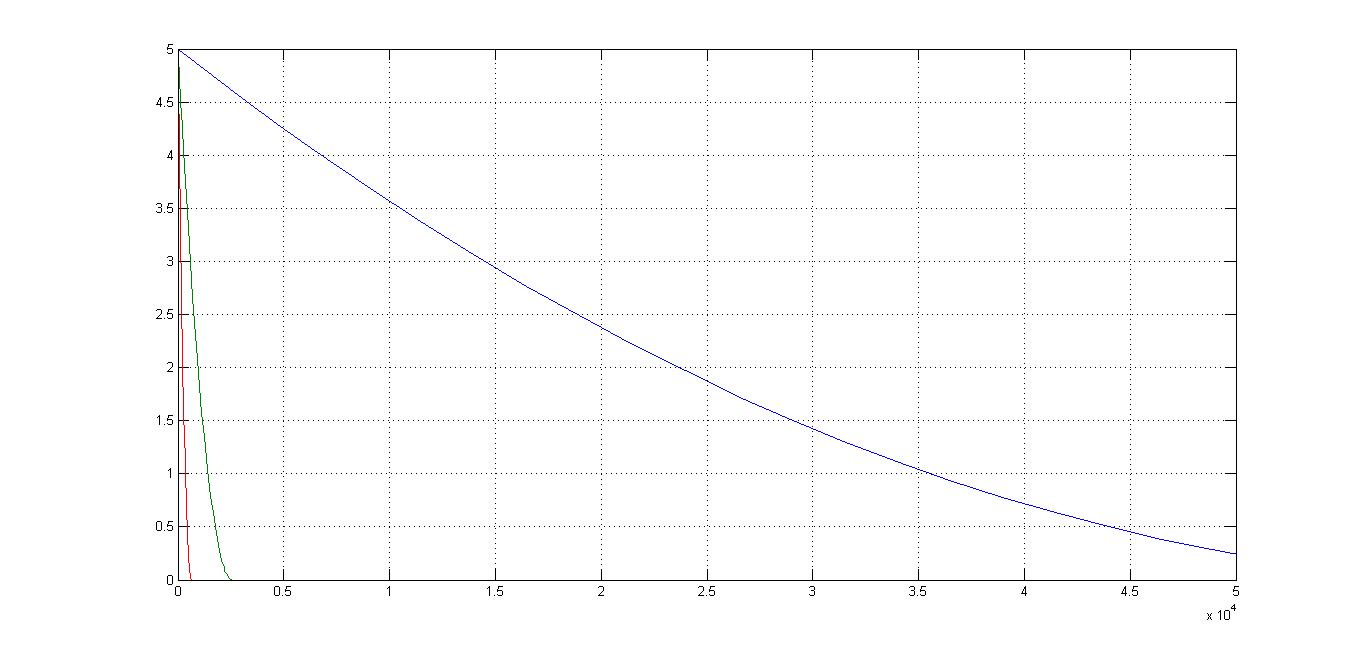
\includegraphics[width=0.8\textwidth]{./p1v2.jpg}
\end{center}
de donde, valores cercanos a 
\begin{lstlisting}
ans =

   1.0e+04 *

    3.6461    0.1446    0.0361

\end{lstlisting}
son los segundos necesarios para la descarga solicitada según el modelo.
\item (20 pt) En un rutero llamado \texttt{p2v2.m}
\begin{enumerate}
\item Grafique la funci\'on
$$
j(x)=\frac{1}{x^2+1}-\frac{1}{2}
$$
en el intervalo $[-3,1]$.
\item Programe el m\'etodo de la secante para que calcule la ra\'iz de de la funci\'on que se encuentra a la derecha de $x=-2$, con una tolerancia de $10^{-8}$.
\end{enumerate}
\textbf{Desarollo:} 
El programa solicitado debe tener instrucciones similares a 
\begin{lstlisting}
j=@(x) 1./(x.^2+1)-1/2;
plot(-3:0.01:1,j(-3:0.01:1));
grid on;
x(1)=-2;
x(2)=-0.5;
tol=1;
i=3;
while tol>10^(-8)
   x(i)=x(i-1)-j(x(i-1))*(x(i-1)-x(i-2))./(j(x(i-1))-j(x(i-2)));
   tol=abs(j(x(i)))
   plot(x(i),j(x(i)));
   i=i+1;
end
format long
x(end)
\end{lstlisting}
\begin{enumerate}
	\item La gr\'afica solicitada es de la forma
    \begin{center}
    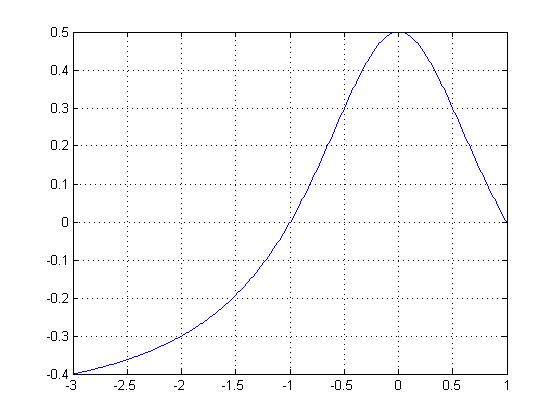
\includegraphics[width=0.8\textwidth]{./p2v2.jpg}
    \end{center}
    \item y el valor aproximado de la ra\'iz es
    \begin{lstlisting}
ans =

  -0.999999999947037
    \end{lstlisting}
\end{enumerate}
\end{enumerate}
\end{document}  